\documentclass[12pt,a4paper]{article}
\usepackage[spanish]{babel}
\usepackage[utf8]{inputenc}
\usepackage{graphicx}
\usepackage[font=footnotesize,labelfont=bf]{caption}
\usepackage[hmargin=1cm,vmargin=2cm]{geometry}
\usepackage{amsmath}
\usepackage{authblk}
\usepackage{url}
\usepackage{float}
\usepackage{multicol}
\usepackage{caption}
\usepackage{sectsty}
\usepackage{fancyhdr}
\usepackage{booktabs} %Agrego líneas a las tablas

\renewcommand{\baselinestretch}{1.5}
\renewcommand\spanishtablename{Tabla}

%Estilo
\sectionfont{\large}
%\pagestyle{fancy}
\renewcommand{\headrulewidth}{0pt}
\newcommand{\comment}[1]{} %Para hacer comentarios


\begin{document}

{\scshape\Huge Perfilador de haz \par}

{\Large Proyecto SOMA \par}

%
\includegraphics[width=0.5\textwidth]{fig/logo}

\section{Especificaciones}

\begin{table}[H]
  \centering
  \begin{tabular}{|c|c|}
    \hline
    Diametro máximo de haz &  8 mm \\ \hline
    Diametro mínimo de haz &  0,5 mm\\ \hline
    Altura del eje óptico   &  5 cm\\ \hline
    Distancia del soporte al eje óptico &  3 cm\\ \hline
  \end{tabular}
  \caption{Especificaciones del haz y dimensiones mínimas}
  \label{tab:perfilador_mecanica}
\end{table}

\begin{table}[H]
  \centering
  \begin{tabular}{|c|c|}
    \hline
    Setup &  Observaciones \\ \hline
    Riel Thorlabs & \footnotesize En eje horizontal se necesita un poste \\ \hline
    Cage Thorlabs mayor a 30mm &   \\ \hline
  \end{tabular}
  \caption{Setups testeados}
  \label{tab:perfilador_setup}
\end{table}


\begin{table}[H]
  \centering
  \begin{tabular}{|c|c|}
    \hline
    Velocidad del motor &  20 rps \\ \hline
    Torque del motor    &  1.4Ncm \\ \hline
  \end{tabular}
  \caption{Detalles del motor y adquisición}
  \label{tab:electronica_adq}
\end{table}


\section{Electrónica}

\begin{table}[H]
  \centering
  \begin{tabular}{|c|c|}
    \hline
    Fuente &  $V > 8\text{V}$, $I>0,5\text{A}$ \\ \hline
    Conector alimentación &  Coaxial 5.5 mm \\ \hline
  \end{tabular}
  \caption{Especificaciones de la fuente de alimentación}
  \label{tab:electronica_tcp}
\end{table}


\begin{table}[H]
  \centering
  \begin{tabular}{|c|c|}
    \hline
    SSID &  WiFi-LEC \\ \hline
    IP (por defecto) &  192.168.0.100 \\ \hline
    Puerto TCP & 23 (Telnet) \\ \hline
    Tiempo de transmisión & 0,5s \\ \hline
  \end{tabular}
  \caption{Específicaciones de conexión}
  \label{tab:electronica_tcp}
\end{table}

En caso de que se haya alterado la IP
\begin{enumerate}
  \item Conectar PC al microcontrolador
  \item Abrir puerto serie creado.
  \item Imprimirá la IP una vez cada 10 s.
\end{enumerate}

\noindent Formato de salida (usar \texttt{telnet} IP\_SENSOR):

\begin{verbatim}
  1;1212
  2;1214
  ...
  Paso_i;Voltaje_i
  ...
  4000;1242
  END
\end{verbatim}

Tiempo de transmisión $\tau \approx 0,5\text{s}$

Preferiblemente usar GUI para obtener ajustes. Ingresar IP del sensor para usarla


\clearpage

\begin{figure}[H]
  \centering
  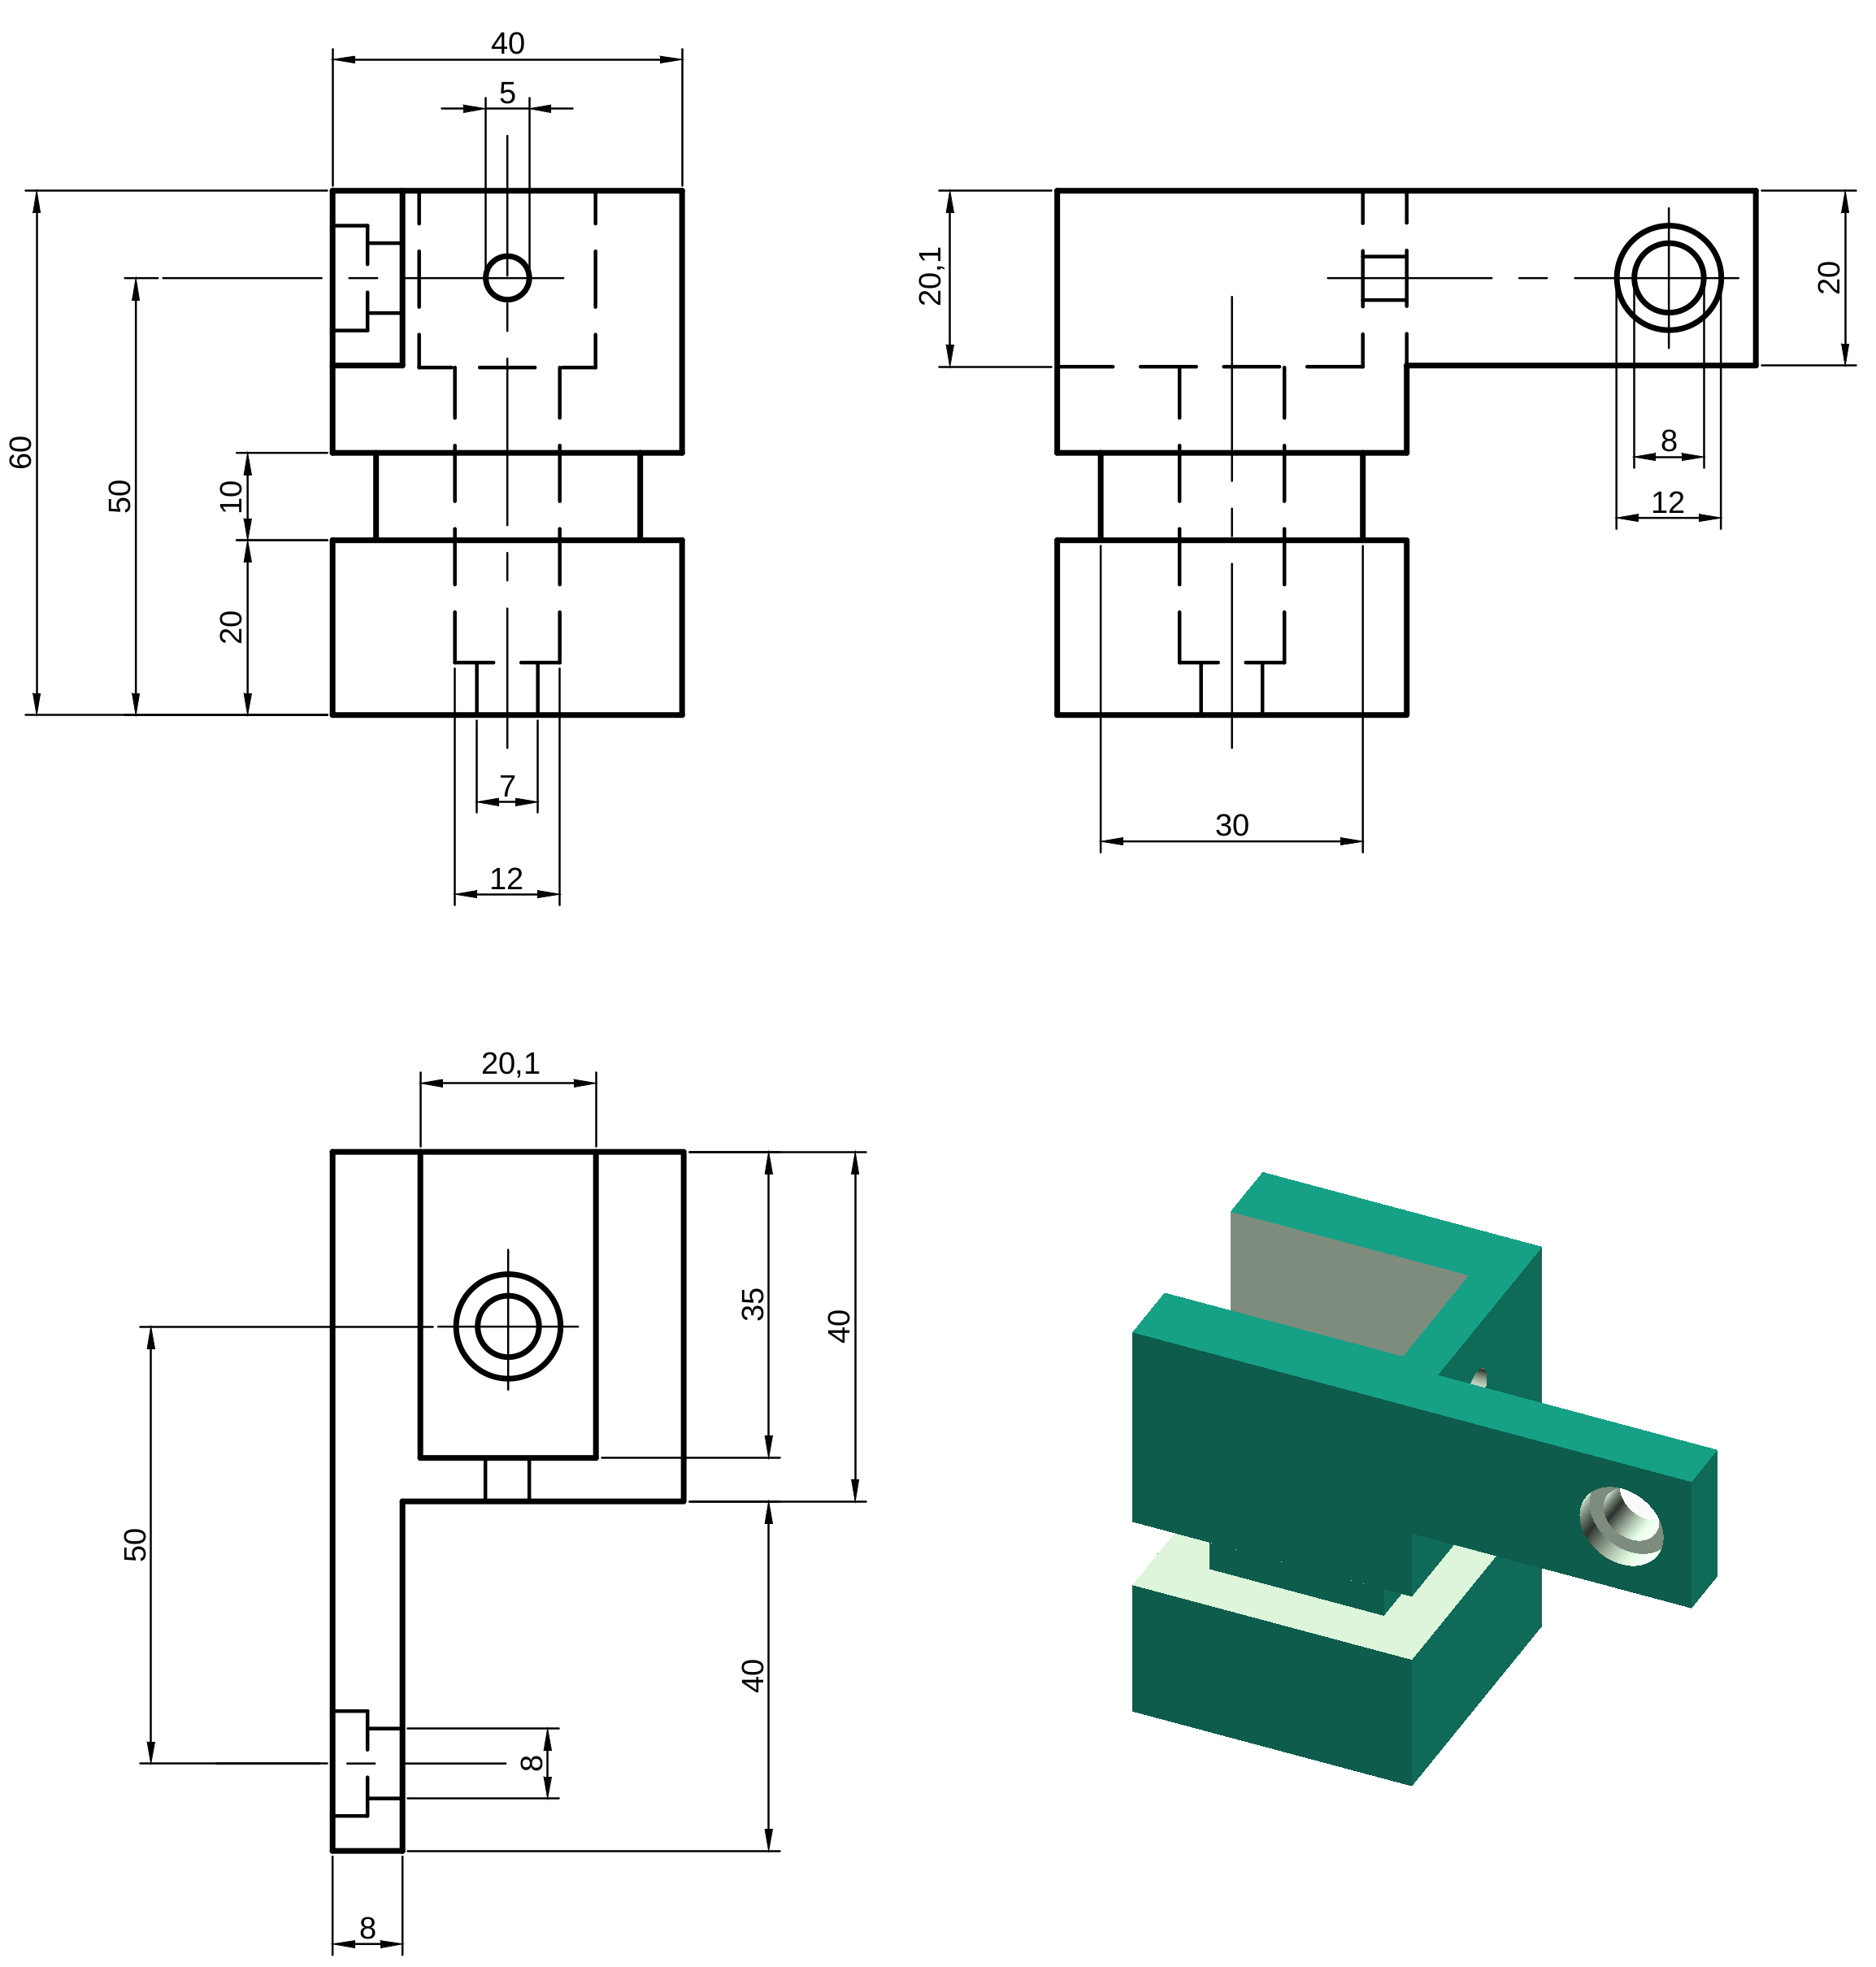
\includegraphics[width=0.8\textwidth]{fig/perfilador}
  \caption{Esquema mecánico del perfilador}
  \label{fig:perfilador}
\end{figure}

\begin{figure}[H]
  \centering
  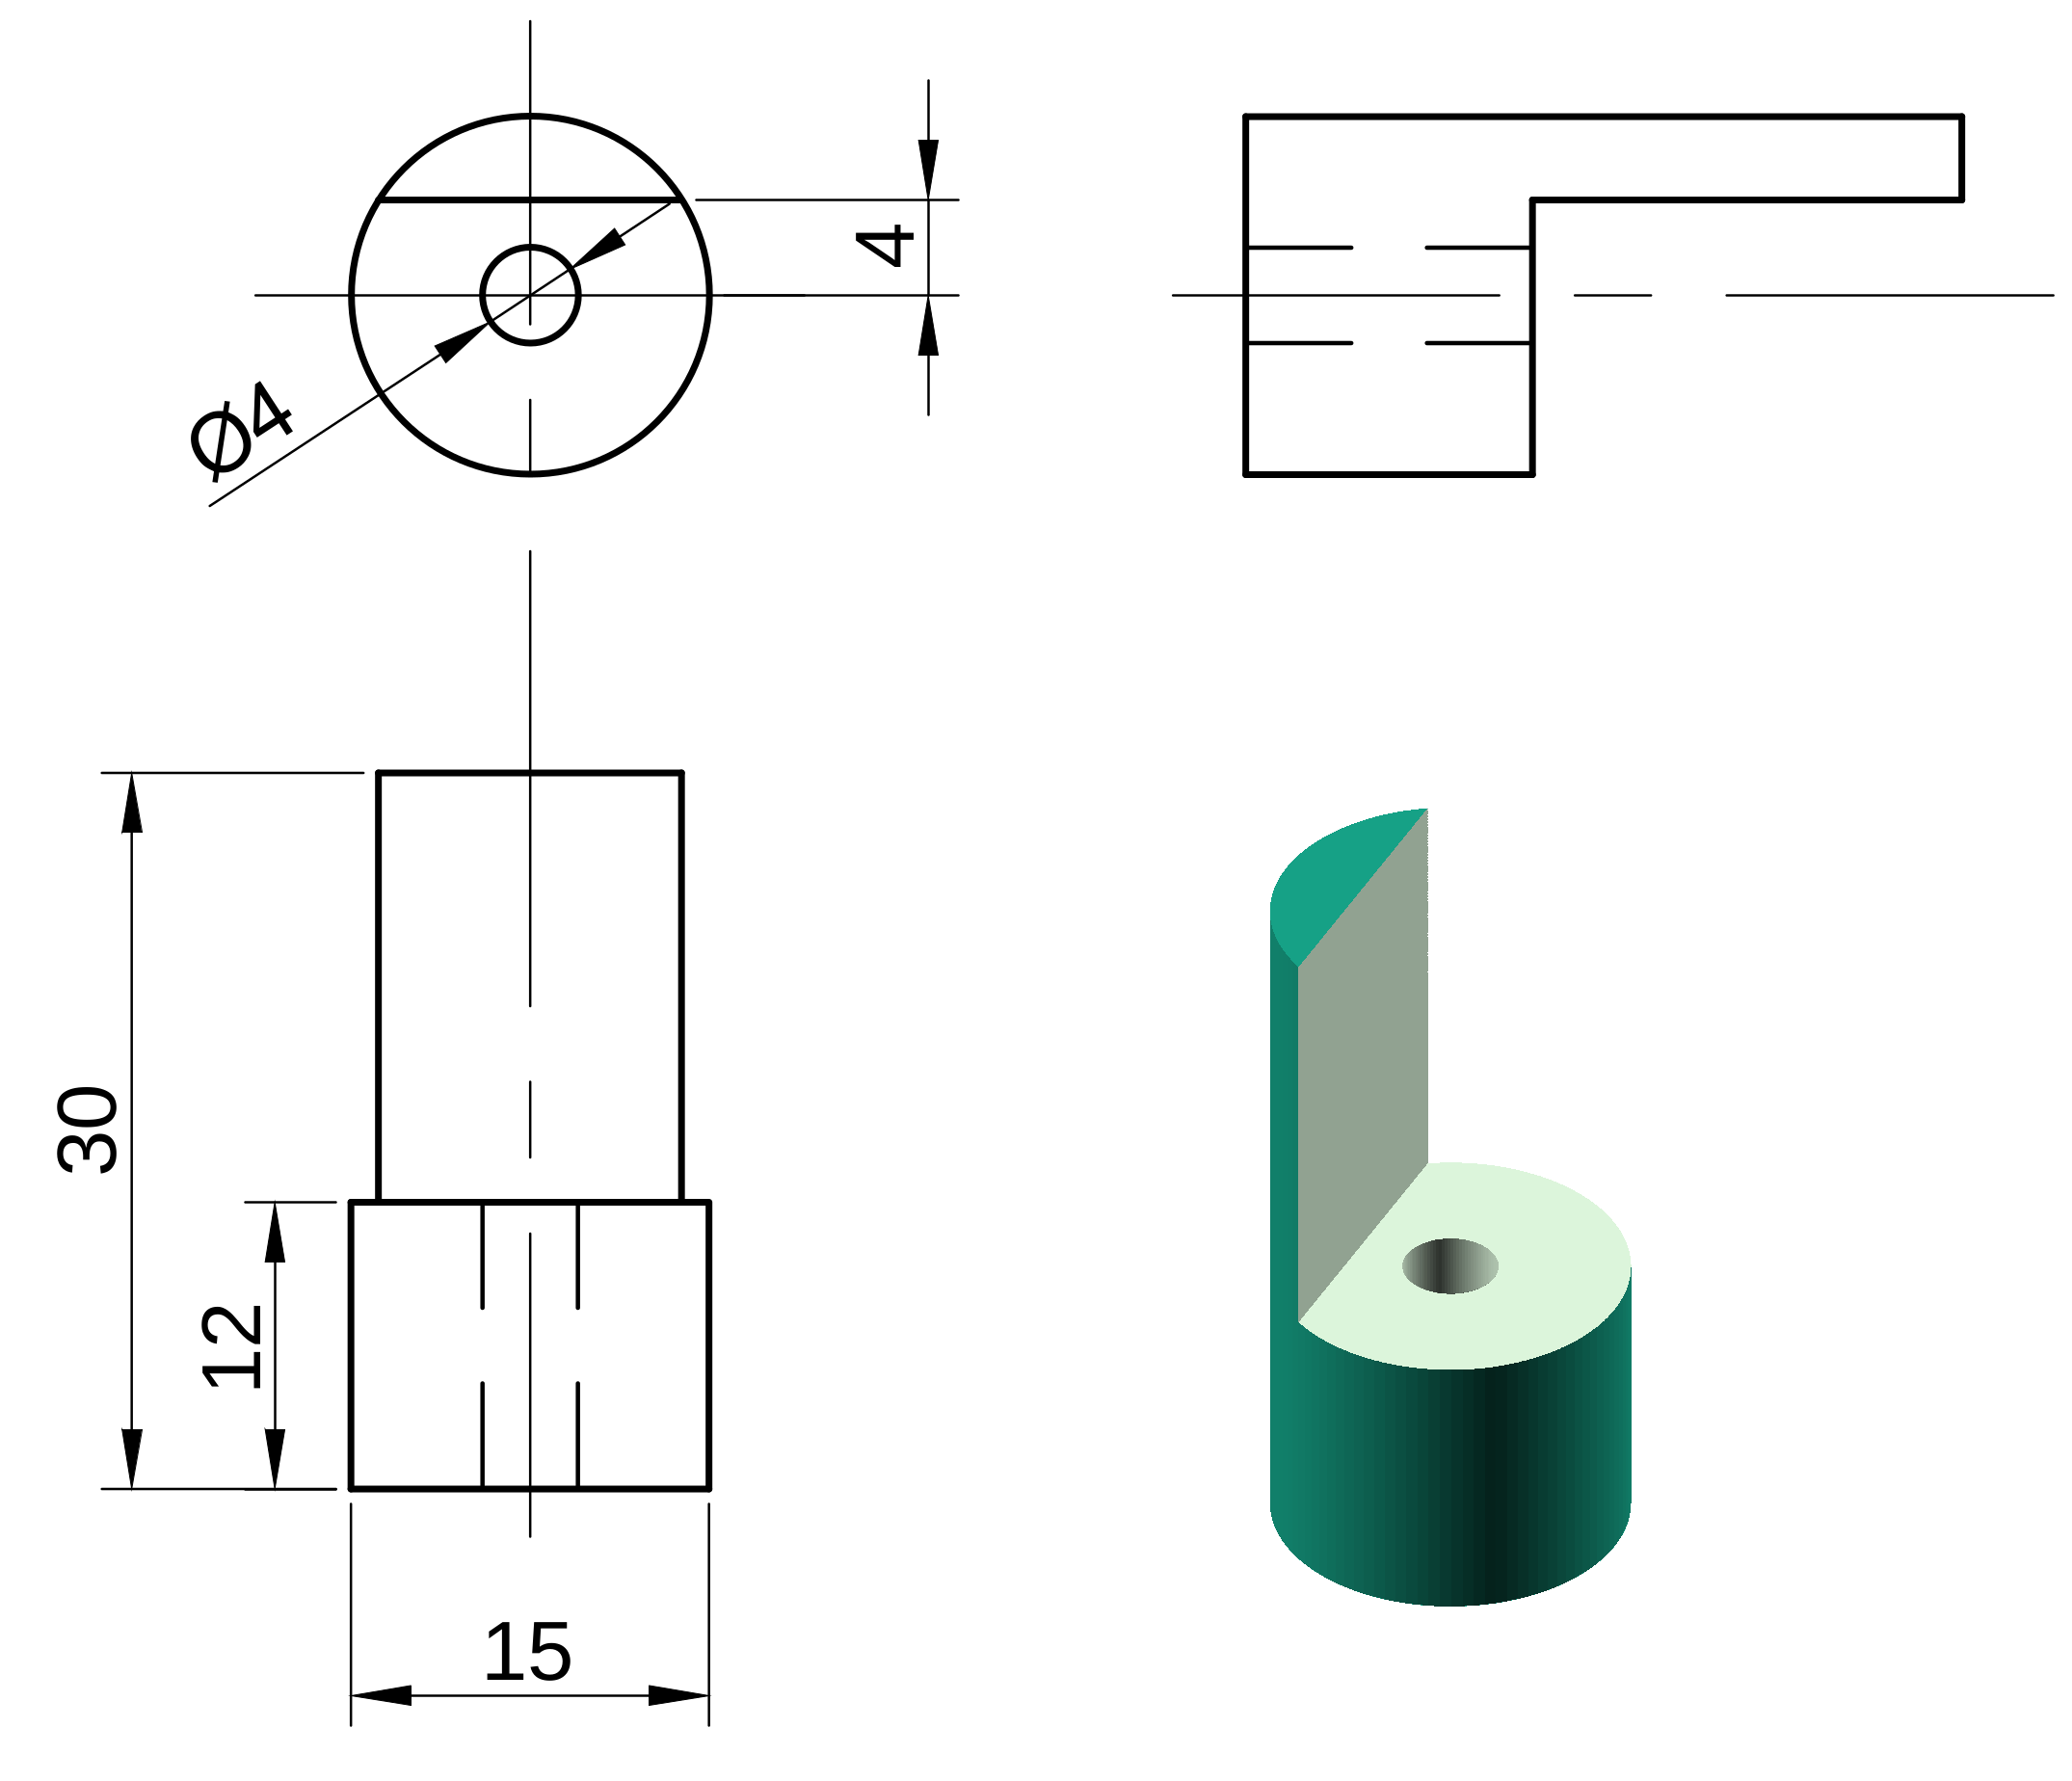
\includegraphics[width=0.4\textwidth]{fig/tambor}
  \caption{Esquema mecánico del tambor}
  \label{fig:perfilador}
\end{figure}

\clearpage

\begin{figure}[H]
  \centering
  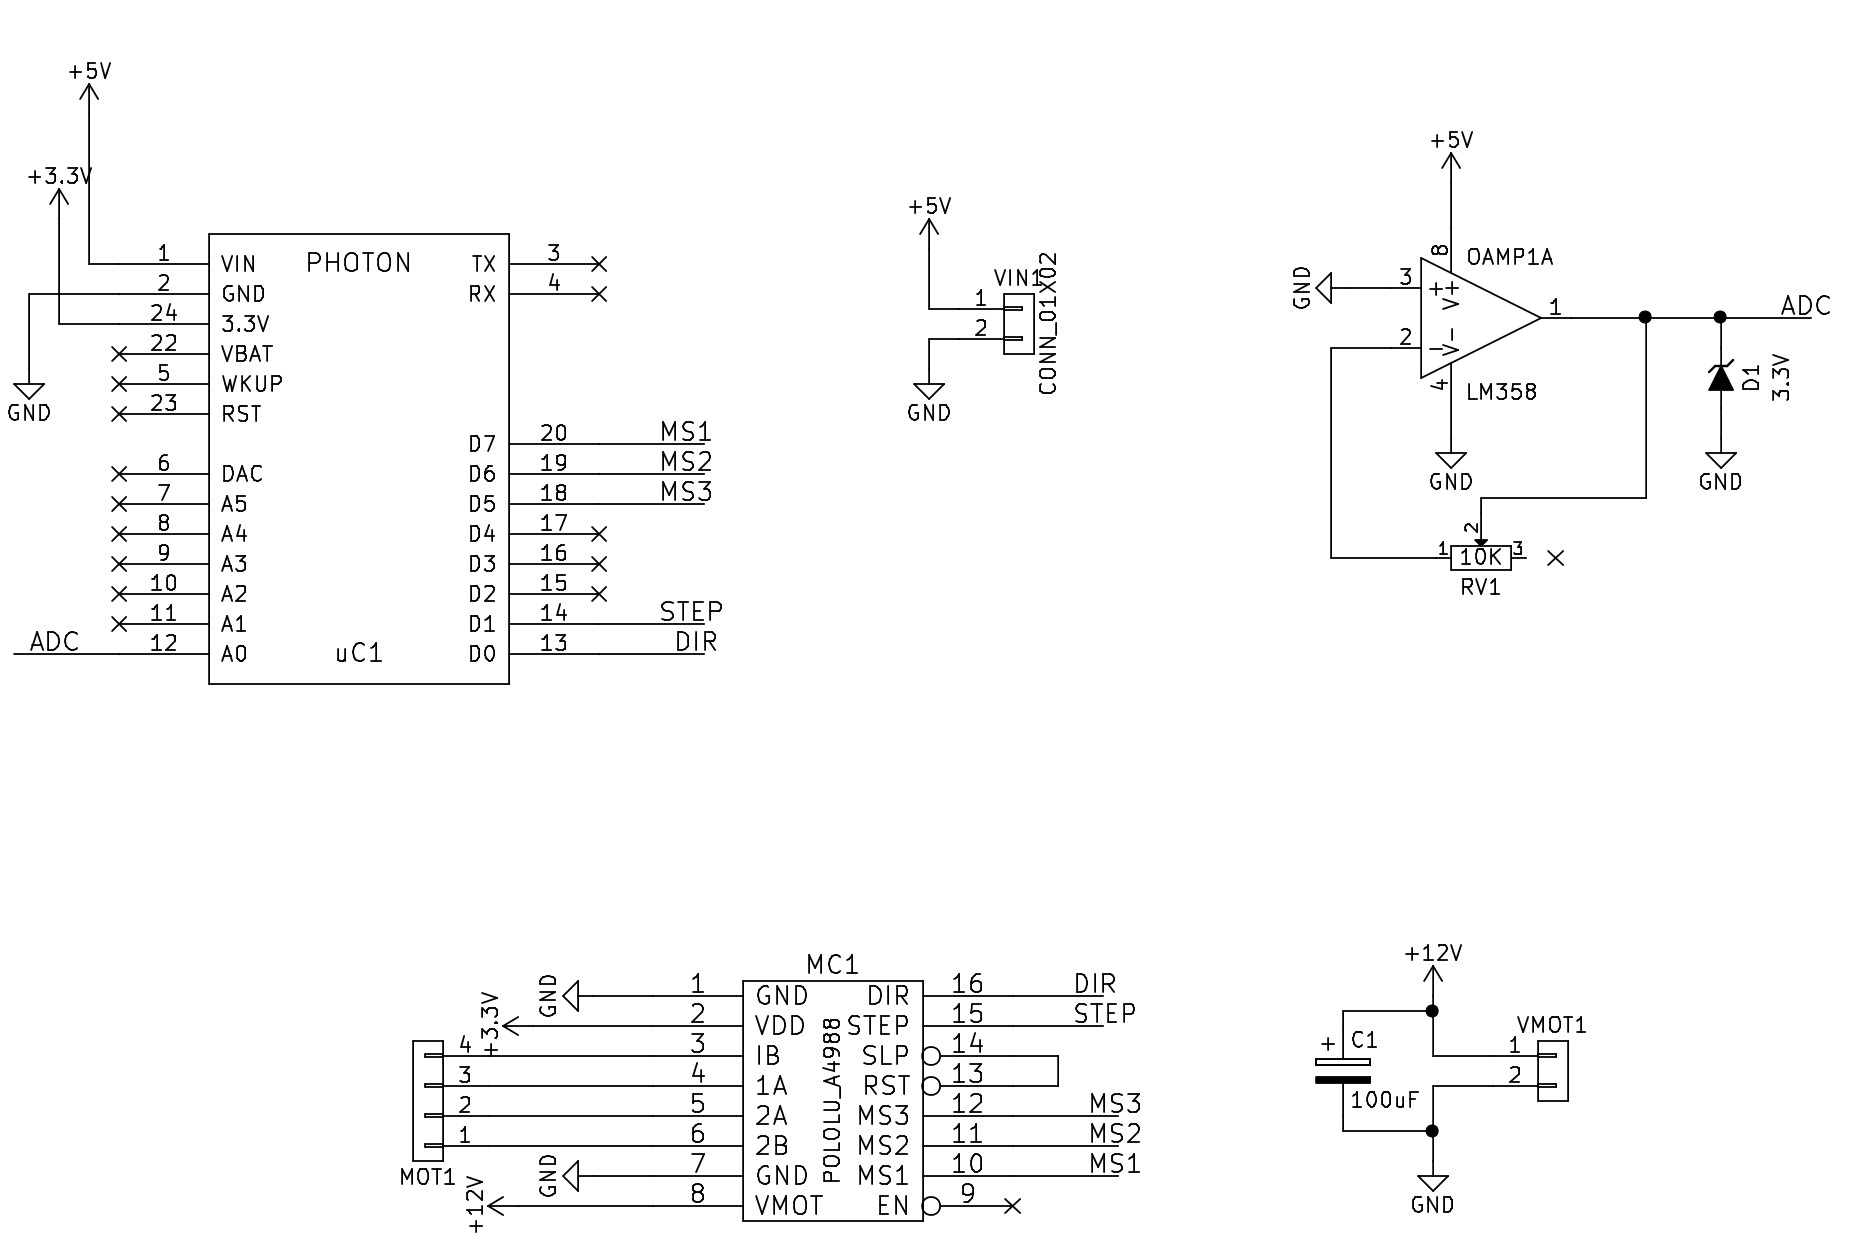
\includegraphics[width=0.9\textwidth]{fig/circuito_esquematico}
  \caption{Esquematico del circuito eléctronico del perfilador.}
  \label{fig:circuito_esquematico}
\end{figure}

\begin{figure}[H]
  \centering
  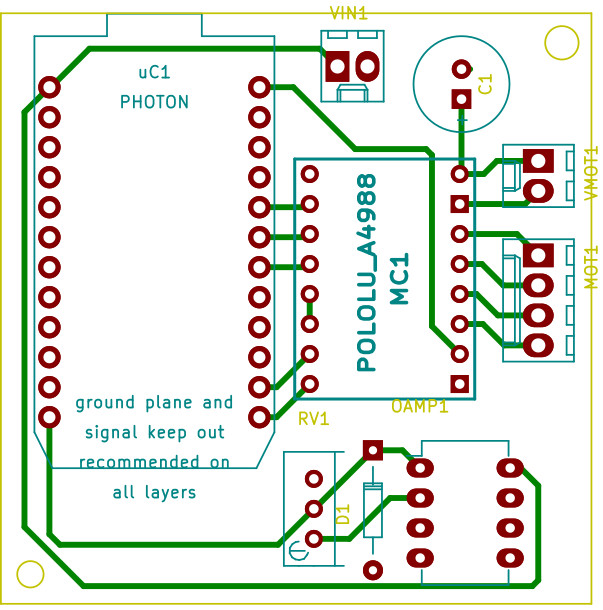
\includegraphics[width=0.4\textwidth]{fig/circuito_pcb}
  \caption{Plano del circuito impreso del perfilador}
  \label{fig:circuito_pcb}
\end{figure}

\end{document}
